\section{Results}
\label{sec:results}

Given a fixed training FLOP budget, \textit{RigL} surpasses existing dynamic sparse training methods over a range of target sparsities, on both CIFAR-10 and 100 (Sections \ref{cifar-10-results}, \ref{cifar-100-results}). By training longer, \textit{RigL} matches or marginally outperforms iterative pruning. However, unlike pruning, its FLOP consumption is constant throughout. This a prime reason for using sparse networks, and makes training larger networks feasible. Finally, as evaluated on CIFAR-10, the original authors' choice of hyper-parameters are close to optimal for multiple target sparsities and initialization schemes (Section \ref{hyperparameter-tuning}).

\jdcomment{Start with a high-level overview of your results. \sout{Does your work support the claims you listed in section 2?} Keep this section as factual and precise as possible, reserve your judgement and discussion points for the next "Discussion" section. 

\textbf{Results reproducing original paper}
For each experiment, say 1) which claim in Section~\ref{sec:claims} it supports, and 2) if it successfully reproduced the associated experiment in the original paper. \sout{how it relates to one of the claims and explain what your result is.} 
For example, an experiment training and evaluating a model on a dataset may support a claim that that model outperforms some baseline.
Logically group related results into sections.} 

\subsection{WideResNet-22 on CIFAR-10}\label{cifar-10-results}

\begin{table}[t]
    \captionsetup{aboveskip=\tableaboveskip,belowskip=\tablebelowskip}
    \caption{\textbf{WideResNet-22-2 on CIFAR10}, tabulated for two density $(1-s)$ values. We group methods by their FLOP requirement and in each group, we mark the best accuracy in bold. Similar to \citet{rigl}, we assume that algorithms utilize sparsity during training. All results are obtained by methods implemented in our unified codebase.}
    \label{tab:cifar10-main-results}
    \centering
    
    \begin{tabular}{ c cc cc }
    \toprule
    \multirow{3}{*}{\textbf{Method}}& 
    \multicolumn{2}{c}{$\mathbf{1 - s=0.1}$} & \multicolumn{2}{c}{$\mathbf{1 - s=0.2}$} \\
    \cmidrule(lr){2-3} \cmidrule(lr){4-5}
    {} & 
    \makecell{Accuracy $\uparrow$ \\ (Test)}  & \makecell{FLOPs $\downarrow$  \\ (Train, Test)} &
    \makecell{Accuracy $\uparrow$ \\ (Test)}  & \makecell{FLOPs $\downarrow$  \\ (Train, Test)} \\
    \midrule
    Small Dense & 
    {89.0 $\pm$ 0.35} & {0.11x, 0.11x} & 
    {91.0 $\pm$ 0.07} & {0.20x, 0.20x} \\
    
    Static & 
    {89.1 $\pm$ 0.17} & {0.10x, 0.10x} & 
    {91.2 $\pm$ 0.16} & {0.20x,0.20x} \\

    SET &
    {91.3 $\pm$ 0.47} & {0.10x, 0.10x} & 
    \textbf{92.7 $\pm$ 0.28} & {0.20x, 0.20x} \\
    
    \textbf{RigL} &
    \textbf{91.7 $\pm$ 0.18} & {0.10x, 0.10x} &
    {92.6 $\pm$ 0.10} & {0.20x, 0.20x} \\
    \midrule
    
    SET (ERK)&
    {92.2 $\pm$ 0.04} & {0.17x, 0.17x} &
    {92.9 $\pm$ 0.16} & {0.35x, 0.35x} \\
    
    \textbf{RigL (ERK)} &
    \textbf{92.4 $\pm$ 0.06} & {0.17x, 0.17x} &
    \textbf{93.1 $\pm$ 0.09} & {0.35x, 0.35x} \\
    \midrule
    {Static\textsubscript{$2 \times$}} &
    {89.15 $\pm$ 0.17} & {0.20x, 0.10x} &
    {91.2 $\pm$ 0.16} & {0.40x, 0.20x} \\
    
    Lottery & 
    {90.4 $\pm$ 0.09} & {0.45x, 0.13x} & 
    {92.0 $\pm$ 0.31} & {0.68x,0.27x} \\
    
    {SET\textsubscript{$2 \times$}} &
    {83.3 $\pm$ 15.33} & {0.20x, 0.10x} &
    {93.0 $\pm$ 0.22} & {0.41x, 0.20x} \\
    
    SNFS & 
    {92.4 $\pm$ 0.43} & {0.51x, 0.27x} & 
    {92.7 $\pm$ 0.20} & {0.66x, 0.49x} \\ 
    
    SNFS (ERK)& 
    {92.2 $\pm$ 0.2} & {0.52x, 0.28x} & 
    {92.8 $\pm$ 0.07} & {0.66x, 0.49x} \\
    
    {SNFS\textsubscript{$2 \times$}} &
    {92.3 $\pm$ 0.33} & {1.02x, 0.27x} &
    {93.2 $\pm$ 0.14} & {1.32x, 0.98x} \\
    
    {RigL\textsubscript{$2 \times$}} &
    {92.3 $\pm$ 0.25} & {0.20x, 0.10x} &
    {93.0 $\pm$ 0.21} & {0.41x, 0.20x} \\
    
    % {RigL\textsubscript{$3 \times$}} &
    % {92.5 $\pm$ 0.11} & {0.30x, 0.10x} &
    % {93.2 $\pm$ 0.20} & {0.61x, 0.20x} \\
    
    {Pruning} & 
    {92.6 $\pm$ 0.08} & {0.32x,0.13x} & 
    {93.2 $\pm$ 0.27} & {0.41x,0.27x} \\ 
    
    \textbf{RigL\textsubscript{$2 \times$} (ERK)} &
    \textbf{92.7 $\pm$ 0.37} & {0.34x, 0.17x} &
    \textbf{93.3 $\pm$ 0.09} & {0.70x, 0.35x} \\
    \midrule
    
    \textbf{Dense Baseline} &
    \textbf{93.4 $\pm$ 0.07} & {9.45e8, 3.15e8} &
    \textbf{-} & {-} \\
    \bottomrule
    
    \end{tabular}
\end{table}
   
Results on the CIFAR-10 dataset are provided in Table \ref{tab:cifar10-main-results}. Tabulated metrics are averaged across 3 random seeds and reported with their standard deviation. All sparse networks use random initialization, unless indicated otherwise.

While SET improves over the performance of static sparse networks and small-dense networks, methods utilizing gradient information (SNFS, \textit{RigL}) obtain better test accuracies. SNFS can outperform \textit{RigL}, but requires a much larger training budget, since it (a) requires dense gradients at each training step, (b) redistributes layer-wise sparsity during mask updates. For all sparse methods, excluding SNFS, using ERK initialization improves performance, but with increased FLOP consumption. We calculate theoretical FLOP requirements in a manner similar to \citet{rigl} (exact details in the supplementary material). 

Figure \ref{fig:cifar10-main-results} contains test accuracies of select methods across two additional sparsity values: ($0.5, 0.95$). At lower sparsities (higher densities), \textit{RigL} matches the performance of the dense baseline. Performance further improves by training for longer durations. Particularly, training \textit{RigL} (ERK) twice as long at 90\% sparsity exceeds the performance of iterative pruning while requiring similar theoretical FLOPs. This validates the original authors' claim that \textit{RigL} (a sparse-to-sparse training method) outperforms pruning (a dense-to-sparse training method). 

\begin{figure}[!t]
    \centering
    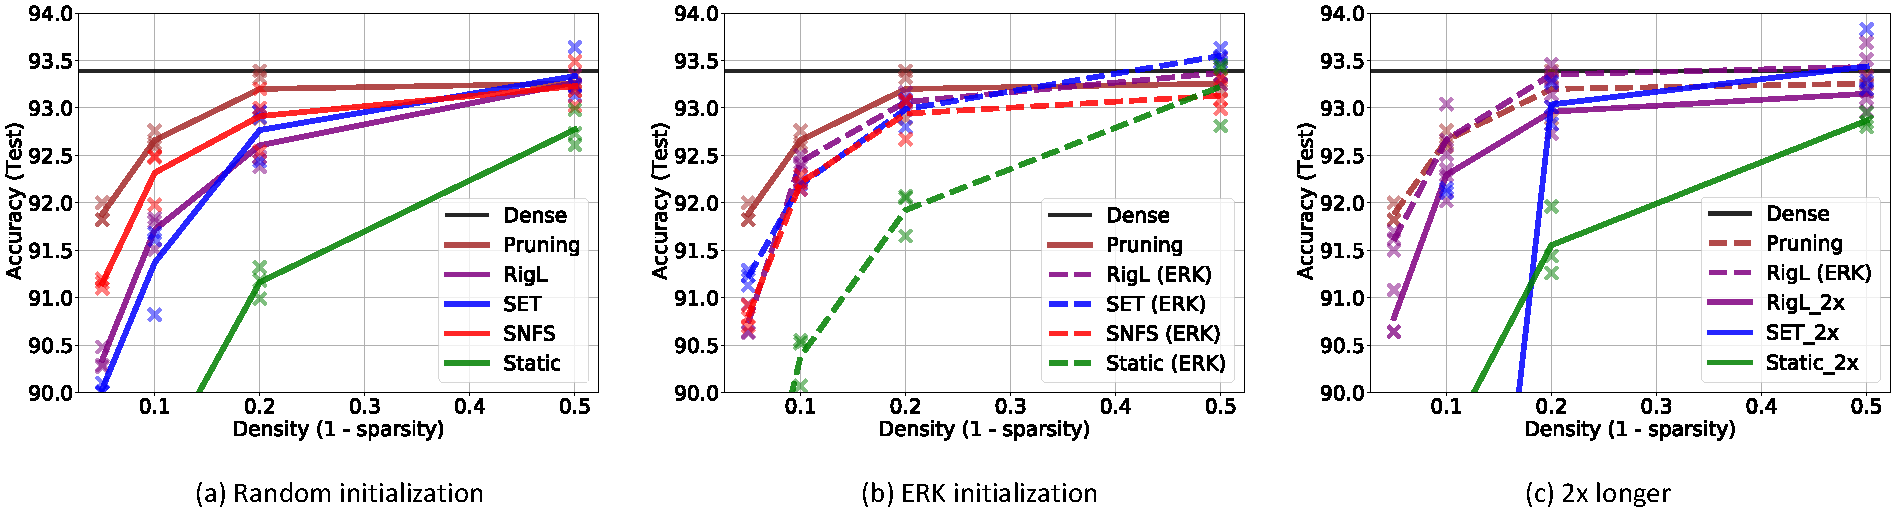
\includegraphics[width=1\textwidth]{../openreview/figs/cifar10_main.pdf}
    \captionsetup{aboveskip=\figureaboveskip,belowskip=\figurebelowskip}
    \caption{\textbf{Test Accuracy vs Sparsity on CIFAR-10,} plotted for Random initialization \textbf{(left)}, ERK initialization \textbf{(center)}, and for training $2\times$ longer \textbf{(right)}. Owing to random growth, SET can be unstable when training for longer durations with higher sparsities. Overall, \textit{RigL}\textsubscript{$2 \times$} (ERK) achieves highest test accuracy.}
    \label{fig:cifar10-main-results}
\end{figure}
\subsection{ResNet-50 on CIFAR100}\label{cifar-100-results}

\begin{tabularx}{\textwidth}[hb]{*{2}{>{\centering\arraybackslash}X}}
    \centering
    \captionsetup{labelformat=andfigure,width=1.1\linewidth,aboveskip=7pt,belowskip=0pt}
    \captionlistentry[figure]{entry for figure}
    \label{fig:cifar100-main-results}
    
    \captionof{table}{\textbf{Benchmarking sparse ResNet-50s on CIFAR-100,} tabulated by performance and cost \textbf{(below)}, and plotted across densities \textbf{(right)}. In each group below, \textit{RigL} outperforms or matches existing sparse-to-sparse and dense-to-sparse methods. Notably, \textit{RigL}\textsubscript{$3\times$} at 90\% sparsity and \textit{RigL}\textsubscript{$2\times$} at 80\% sparsity surpass iterative pruning with similar FLOP consumption. \textit{RigL}\textsubscript{$2\times$} (ERK) further improves performance but requires a larger training budget. }
    \resizebox{1.15\linewidth}{!}{%
\begin{tabular}{ c cc cc }
\toprule
\multirow{3}{*}{\textbf{Method}}& 
\multicolumn{2}{c}{$\mathbf{1 - s=0.1}$} & \multicolumn{2}{c}{$\mathbf{1 - s=0.2}$} \\
\cmidrule(lr){2-3} \cmidrule(lr){4-5}
{} & 
\makecell{Accuracy $\uparrow$ \\ (Test)}  & \makecell{FLOPs $\downarrow$  \\ (Train, Test)} &
\makecell{Accuracy $\uparrow$ \\ (Test)}  & \makecell{FLOPs $\downarrow$  \\ (Train, Test)} \\
\midrule
Static & 
{69.7 $\pm$ 0.42} & {0.10x, 0.10x} & 
{72.3 $\pm$ 0.30} & {0.20x,0.20x} \\

Small Dense & 
{70.8 $\pm$ 0.22} & {0.11x, 0.11x} & 
{72.6$\pm$ 0.93} & {0.20x, 0.20x} \\

SET &
{71.4 $\pm$ 0.35} & {0.10x, 0.10x} & 
{73.4 $\pm$ 0.45} & {0.20x, 0.20x} \\

\textbf{RigL} &
\textbf{71.8 $\pm$ 0.33} & {0.10x, 0.10x} &
\textbf{73.5 $\pm$ 0.04} & {0.20x, 0.20x} \\
\midrule

Static (ERK) & 
{71.5 $\pm$ 0.18} & {0.22x, 0.22x} & 
{73.2 $\pm$ 0.39} & {0.38x, 0.38x} \\

SET (ERK)&
{72.3 $\pm$ 0.39} & {0.22x, 0.22x} &
\textbf{73.5 $\pm$ 0.25} & {0.38x, 0.38x} \\

\textbf{RigL (ERK)} &
\textbf{72.6 $\pm$ 0.37} & {0.23x, 0.22x} &
{73.4 $\pm$ 0.15} & {0.38x, 0.38x} \\
\midrule

SNFS & 
{72.3 $\pm$ 0.20} & {0.58x, 0.37x} & 
{73.9 $\pm$ 0.20} & {0.70x, 0.55x} \\ 

SNFS (ERK)& 
{73.0 $\pm$ 0.33} & {0.59x, 0.38x} & 
{73.9 $\pm$ 0.27} & {0.69x, 0.54x} \\

{Pruning} & 
{73.1 $\pm$ 0.32} & {0.36x,0.11x} & 
{73.8 $\pm$ 0.23} & {0.45x,0.25x} \\ 

{RigL\textsubscript{$2 \times$}} &
{73.1 $\pm$ 0.71} & {0.20x, 0.10x} &
{74.0 $\pm$ 0.24} & {0.41x, 0.20x} \\

{Lottery} &
{73.6 $\pm$ 0.32} & {0.62x,0.11x} & 
{74.2 $\pm$ 0.41} & {0.81x,0.25x} \\

\textbf{RigL\textsubscript{$3 \times$}} &
\textbf{73.7 $\pm$ 0.16} & {0.30x, 0.10x} &
{74.2 $\pm$ 0.23} & {0.61x, 0.20x} \\

\textbf{RigL\textsubscript{$2 \times$} (ERK)} &
{73.6 $\pm$ 0.05} & {0.46x, 0.22x} &
\textbf{74.4 $\pm$ 0.10} & {0.76x, 0.38x} \\

\midrule

\textbf{Dense Baseline} &
\textbf{74.7 $\pm$ 0.38} & {7.77e9, 2.59e9} &
\textbf{-} & {-} \\
\bottomrule

\end{tabular}%
}

    \label{tab:cifar100-main-results}  
&
    \centering
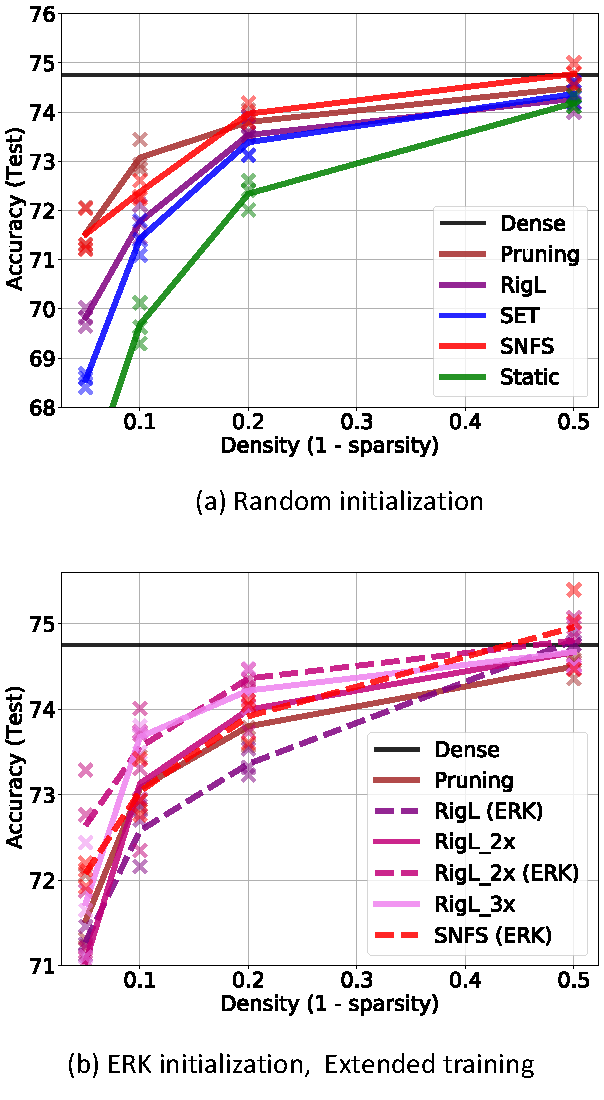
\includegraphics[width=0.66\linewidth,valign=t]{../openreview/figs/cifar100_main.pdf}
\end{tabularx}

We see similar trends when training sparse variants of ResNet-50 on the CIFAR-100 dataset (Table \ref{tab:cifar100-main-results}, metrics reported as in Section \ref{cifar-10-results}). We also include a comparison against sparse networks trained with the Lottery Ticket Hypothesis (\citet{frankle2018lottery}) in Table \ref{tab:cifar100-main-results}---we obtain tickets with a commensurate performance for sparsities lower than 80\%. Finally, the choice of initialization scheme affects the performance and FLOP consumption by a greater extent than the method used itself, with the exception of SNFS (groups 1 and 2 in Table \ref{tab:cifar100-main-results}). 


\subsection{Hyperparameter Tuning}\label{hyperparameter-tuning}

\begin{table}[th]
    \captionsetup{aboveskip=\tableaboveskip,belowskip=\tablebelowskip}
    \caption{\textbf{Reference vs Optimal $(\alpha, \Delta T)$ on CIFAR-10.} Optimal hyperparameters are obtained by tuning with a TPE sampler in Optuna. The difference between the reference and optimal performance is small, indicating that there is not a significant benefit in tuning $(\alpha, \Delta T)$ individually for each initialization and sparsity configuration.}
    \label{tab:effect-alpha-deltaT}
    \centering
    
    \begin{tabular}{ c c  cc  cc}
    \toprule
    \multirow{3}{*}{\textbf{Initialization}} & \textbf{Density} & 
    \multicolumn{2}{c}{\textbf{Reference}} & \multicolumn{2}{c}{\textbf{Optimal}} \\
    \cmidrule(lr){2-2} \cmidrule(lr){3-4} \cmidrule(lr){5-6}
    {} & {$(1-s)$} & 
    {$(\alpha, \Delta T)$} & \makecell{Accuracy $\uparrow$ \\ (Test)} & 
    {$(\alpha, \Delta T)$} & \makecell{Accuracy $\uparrow$ \\ (Test)} \\
    \midrule
    
    Random & 0.1 & 
    {0.3, 100} & {91.7 $\pm$ 0.18} &  
    {0.197, 50} & \textbf{91.8 $\pm$ 0.17} \\
    
    Random & 0.2 & 
    {0.3, 100} & {92.6 $\pm$ 0.10} &  
    {0.448, 150} & \textbf{92.8 $\pm$ 0.16} \\
    
    Random & 0.5 & 
    {0.3, 100} & \textbf{93.3 $\pm$ 0.07} &  
    {0.459, 550} & \textbf{93.3 $\pm$ 0.18} \\
    \midrule
    
    ERK & 0.1 & 
    {0.3, 100} & \textbf{92.4 $\pm$ 0.06} &  
    {0.416, 200} & \textbf{92.4 $\pm$ 0.23} \\
    
    ERK & 0.2 & 
    {0.3, 100} & \textbf{93.1 $\pm$ 0.09} &  
    {0.381, 950} & \textbf{93.1 $\pm$ 0.21} \\
    
    ERK & 0.5 & 
    {0.3, 100} & {93.4 $\pm$ 0.14} &  
    {0.287, 500} & \textbf{93.8 $\pm$ 0.06} \\
    \hline

    \end{tabular}
    
    \label{tab:replication_verify}
\end{table}

\subsubsection{$(\alpha, \Delta T)$ vs Sparsities} To understand the impact of the two additional hyperparameters included in \textit{RigL}, we use a Tree of Parzen Estimator (TPE sampler, \citet{TPE_Bergstra}) via Optuna to tune $(\alpha, \Delta T)$. We do this for sparsities $(1 - s) \in \{0.1,0.2,0.5\}$, and a fixed learning rate of $0.1$. Additionally, we set the sampling domain for $\alpha$ and $\Delta T$ as $[0.1,0.6]$ and $\{50,100, 150,...,1000\}$ respectively. We use 15 trials for each sparsity value, with our objective function as the validation accuracy averaged across 3 random seeds.

\begin{figure}[!b]
    \centering
    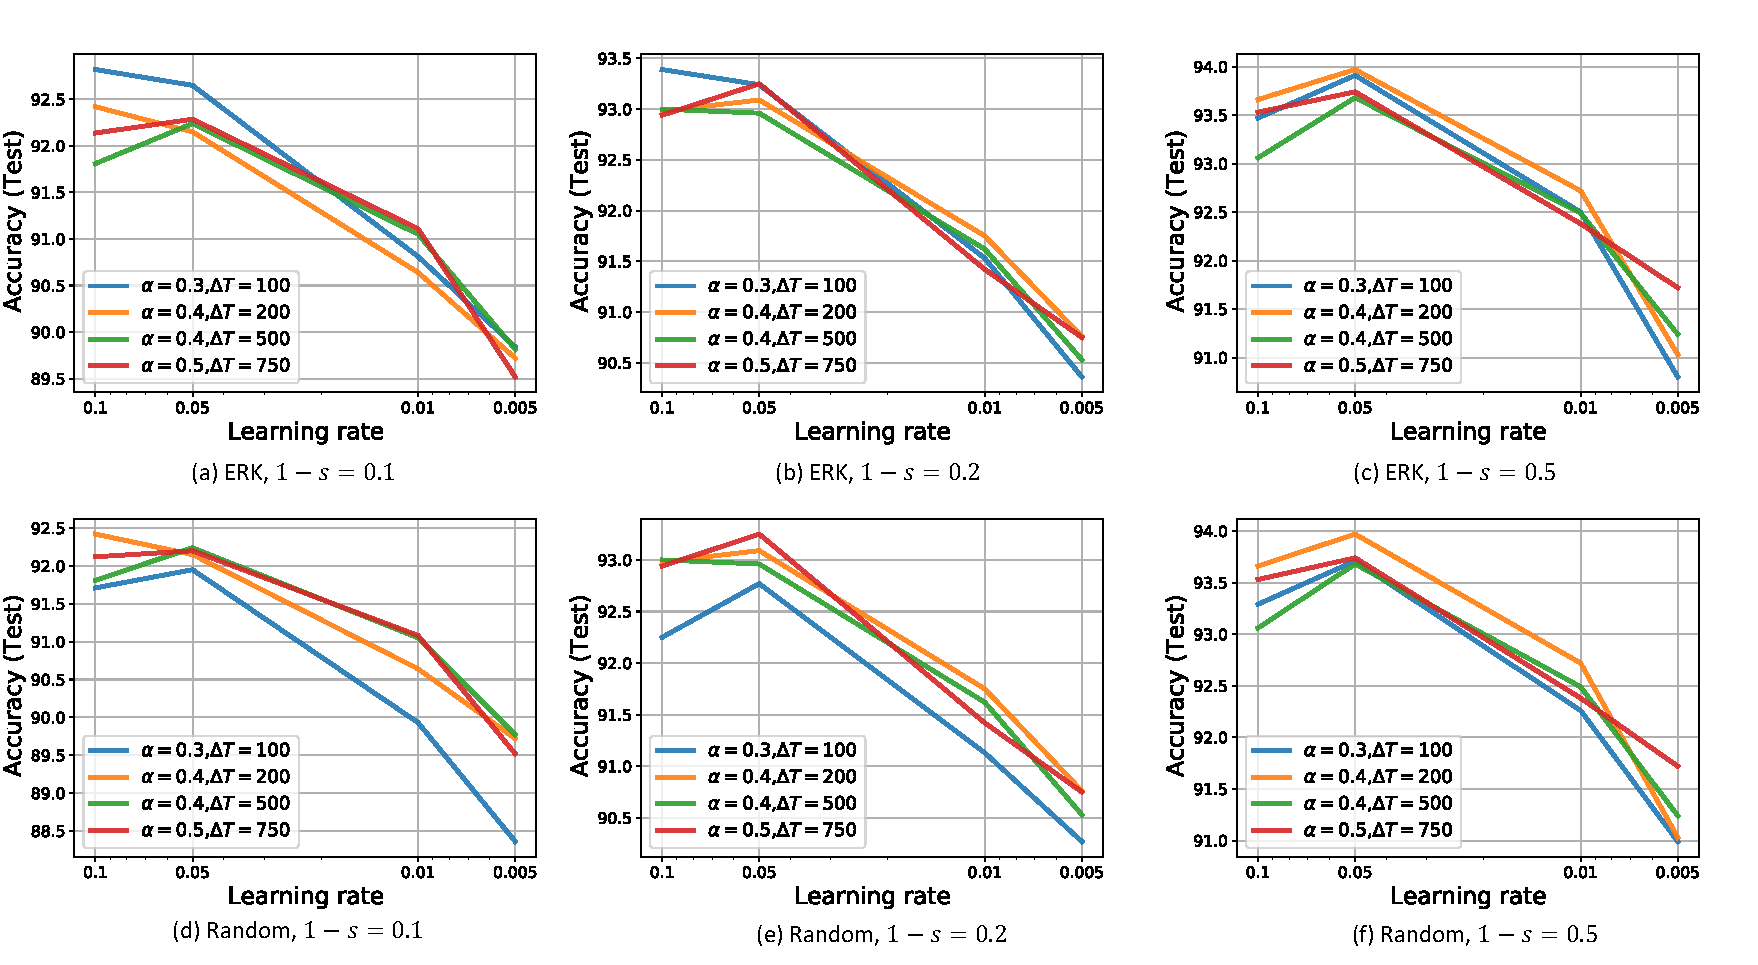
\includegraphics[width=\textwidth]{../openreview/figs/lr_sweep.pdf}
    \captionsetup{aboveskip=\figureaboveskip,belowskip=\figurebelowskip}
    \caption{\textbf{Learning Rate vs Sparsity on CIFAR-10.} Runs using a learning rate $> 0.1$ do not converge and are not plotted here. There is little benefit in tuning the learning rate for each sparsity, and $0.1, 0.05$ are good choices overall.}
    \label{fig:lr-sweep}
\end{figure}

Table \ref{tab:effect-alpha-deltaT} shows the test accuracies of tuned hyperparameters. While the reference hyperparameters (original authors, $\alpha=0.3, \Delta T=100$) differ from the obtained optimal hyperparameters, the difference in performance is marginal, especially for ERK initialization. This in agreement with the original paper, which finds $\alpha \in \{0.3, 0.5\}, \Delta T = 100$ to be suitable choices. We include contour plots detailing the hyperparameter trial space in the supplementary material.

\subsubsection{Learning Rate vs Sparsities} We further examine if the final performance improves by tuning the learning rate ($\eta$) individually for each sparsity-initialization pair. We employ a grid search over $\eta \in \{0.1,0.05,0.01,0.005\}$ and $(\alpha, \Delta T) \in \{(0.3, 100), (0.4,200), (0.4, 500), (0.5, 750)\}$. As seen in Figure \ref{fig:lr-sweep}, $\eta = 0.1$ and $\eta = 0.05$ are close to optimal values for a wide range of sparsities and initializations. Since these learning rates also correspond to good choices for the Dense baseline, one can employ similar values when training with \textit{RigL}.



